\documentclass[12pt]{article}
\usepackage[utf8]{inputenc}
\usepackage{amsmath, amssymb}
\usepackage{graphicx}
\usepackage{geometry}
\geometry{a4paper, left=3cm, right=3cm, top=2.5cm, bottom=2.5cm}
\usepackage{setspace}
\usepackage{tocloft}

\begin{document}
	
	% Portada
	\begin{titlepage}
		\centering
		{\scshape\Large UNIVERSIDAD NACIONAL DE INGENIERÍA \par}
		{\scshape\large Facultad de Ingeniería Industrial y de Sistemas Unidad de Posgrado \par}
		{\scshape\large Maestría en Inteligencia Artificial \par}
		\vspace{2cm}
		
\includegraphics[width=0.25\textwidth]{imagenes/logo.png}\par\vspace{1cm}
		
		{\Huge\bfseries Aplicación del Álgebra Lineal en Técnicas de Machine Learning para la Reducción de Dimensiones y Modelado Predictivo en Pandemias \par}
		\vspace{1.5cm}
		{\large\bfseries Trabajo de Investigación \par}
		\vspace{0.5cm}
		{\large Matemática para Machine Learning (MIA 102) Sección “A” | 2025 – I \par}
		\vspace{0.5cm}
		{\large\bfseries Grupo \#7: \par}
		\vspace{0.5cm}
		{\large Koc Góngora, Luis Enrique \par}
		{\large Mancilla Antay, Alex Felipe \par}
		{\large Melendez Garcia, Herbert Antonio \par}
		{\large Paitan Cano, Dennis Jack \par}
		\vfill
		{\large 14 de mayo de 2025 \par}
	\end{titlepage}
	
	\tableofcontents
	\newpage
	
	\onehalfspacing
	
	\section{Resumen y Palabras Clave}
	\noindent
	Este informe presenta una revisión y análisis del artículo \emph{"A Model Based Linear Algebraic Approach for Machine Learning"}. Se describe cómo el álgebra lineal sirve como base matemática para técnicas fundamentales en Machine Learning, incluyendo la Regresión Lineal por Mínimos Cuadrados, Análisis de Componentes Principales (PCA) y Descomposición en Valores Singulares (SVD). El estudio tiene como objetivo evaluar cómo estas herramientas pueden aplicarse a contextos reales como la predicción de necesidades hospitalarias durante la pandemia del COVID-19. Se analizan conceptos como matrices, vectores, autovalores y covarianzas, y se detalla la implementación computacional en Python.

	\vspace{1em}
	\noindent
	\textbf{Palabras clave}: Álgebra Lineal; PCA (Análisis de Componentes Principales); SVD (Descomposición en Valores Singulares); Regresión Lineal; Reducción de Dimensiones; COVID-19; Autovalores; Vectores Propios (Autovectores); Matrices; Covarianza.
	\newpage
	\section{Introducción}
	\noindent
	El artículo de base propone una aproximación matemática basada en el álgebra lineal para resolver problemas en Machine Learning. Esta área de la matemática resulta esencial en la implementación y comprensión de modelos que requieren el manejo eficiente de grandes cantidades de datos. El interés del grupo en este artículo radica en la posibilidad de aplicar estos conceptos teóricos a contextos críticos como la pandemia por COVID-19, donde la toma de decisiones informadas puede salvar vidas. Se destaca el uso de herramientas como PCA y SVD para analizar datos médicos complejos, así como la regresión lineal como modelo predictivo.
	
	\vspace{1em}
	\noindent
	El álgebra lineal, en este sentido, ofrece un lenguaje preciso y estructuras como vectores y matrices que permiten representar grandes volúmenes de datos y transformarlos. Mediante técnicas como la factorización de matrices o el análisis de componentes principales, se pueden identificar patrones, reducir redundancias y obtener predicciones útiles.
	
	\newpage
	\section{Material de Matemática}



\noindent
A continuación se presenta una lista comentada de las herramientas matemáticas y estadísticas empleadas en el artículo \emph{"A Model Based Linear Algebraic Approach for Machine Learning"}:

\begin{itemize}
	\item \textbf{Álgebra Lineal}. Proporciona el marco matemático para representar datos y transformaciones mediante estructuras como matrices y vectores.
	
	\item \textbf{Matrices}. Permiten representar transformaciones lineales y datos multivariados. La multiplicación de matrices se define como:
	\[
	(AB)_{ij} = \sum_k A_{ik} B_{kj}
	\]
	donde $A$ es de tamaño $m \times n$ y $B$ de tamaño $n \times p$.
	
	\item \textbf{Vectores}. Representan datos o características en un espacio $n$-dimensional:
	\[
	\mathbf{v} = \begin{bmatrix} v_1 \\ v_2 \\ \vdots \\ v_n \end{bmatrix}
	\]
	
	\item \textbf{Autovalores y Autovectores}. Dados una matriz cuadrada $A$ y un vector no nulo $x$, se cumplen:
	\[
	A \mathbf{x} = \lambda \mathbf{x}
	\]
	donde $\lambda$ es el autovalor correspondiente a $\mathbf{x}$.
	
	\item \textbf{Matriz de Covarianza}. Mide cómo varían conjuntamente dos variables $X$ e $Y$:
	\[
	\text{cov}(X, Y) = \frac{1}{n} \sum_{i=1}^n (X_i - \bar{X})(Y_i - \bar{Y})
	\]
	
	\item \textbf{Análisis de Componentes Principales (PCA)}. Encuentra nuevas variables (componentes principales) que maximizan la varianza:
	\[
	Y = X W
	\]
	donde $X$ son los datos centrados y $W$ contiene los autovectores.
	
	\item \textbf{Descomposición en Valores Singulares (SVD)}. Factoriza una matriz $A$ como:
	\[
	A = U \Sigma V^T
	\]
	donde $U$ y $V$ son ortogonales y $\Sigma$ es diagonal.
	
	\item \textbf{Regresión Lineal por Mínimos Cuadrados}. Encuentra la recta que minimiza:
	\[
	\sum_{i=1}^n (y_i - (m x_i + b))^2
	\]
	Las fórmulas para $m$ y $b$ se calculan mediante promedios y productos cruzados.
\end{itemize}

\vspace{1em}
\noindent
Cada herramienta contribuye a representar y analizar datos de manera eficiente, permitiendo identificar patrones relevantes y mejorar la capacidad predictiva de los modelos.


\newpage
\section{Fundamentos Teóricos del Material}

\section*{Análisis de Componentes Principales (PCA)}

\noindent
El \textbf{Análisis de Componentes Principales (PCA)} es una técnica estadística que busca \emph{reducir la dimensionalidad} de un conjunto de datos, manteniendo la mayor parte de su \textbf{varianza}. Se basa en encontrar \emph{nuevas variables} (componentes principales) que son combinaciones lineales de las originales y están ordenadas por la cantidad de varianza que explican.

\vspace{1em}
\noindent
A continuación se detallan los fundamentos matemáticos que sustentan esta herramienta:

\subsection*{1. Datos centrados}

Dado un conjunto de datos \( X \in \mathbb{R}^{n \times p} \) (con \( n \) observaciones y \( p \) variables), el primer paso es \textbf{centrar} los datos:
\[
X_{\text{centrado}} = X - \mathbf{1}_n \bar{x}^T
\]
donde \(\bar{x}\) es el vector de medias de las columnas y \(\mathbf{1}_n\) es un vector columna de unos de dimensión \( n \).

\subsection*{2. Matriz de Covarianza}

La \textbf{matriz de covarianza} \( C \) resume las relaciones lineales entre las variables:
\[
C = \frac{1}{n-1} X_{\text{centrado}}^T X_{\text{centrado}}
\]
donde \( C \in \mathbb{R}^{p \times p} \).

\subsection*{3. Descomposición espectral}

El paso clave consiste en encontrar los \emph{autovalores} y \emph{autovectores} de la matriz de covarianza:
\[
C \mathbf{v}_i = \lambda_i \mathbf{v}_i
\]
donde:
\begin{itemize}
	\item \(\lambda_i\): autovalor asociado (mide la varianza explicada por el componente \( i \)).
	\item \(\mathbf{v}_i\): autovector asociado (dirección del componente principal).
\end{itemize}

Los autovectores forman una base ortonormal:
\[
V = [\mathbf{v}_1, \mathbf{v}_2, \ldots, \mathbf{v}_p]
\]
y los autovalores se ordenan de mayor a menor:
\[
\lambda_1 \geq \lambda_2 \geq \cdots \geq \lambda_p
\]

\subsection*{4. Proyección en componentes principales}

La proyección de los datos originales en los \emph{componentes principales} se obtiene como:
\[
Y = X_{\text{centrado}} V
\]
donde \( Y \in \mathbb{R}^{n \times p} \) son las \emph{coordenadas} de los datos en el nuevo sistema de ejes (componentes principales).

\subsection*{5. Varianza explicada}

Cada \emph{autovalor} indica la cantidad de varianza explicada por el componente correspondiente:
\[
\text{Varianza explicada por } \mathbf{v}_i = \frac{\lambda_i}{\sum_{j=1}^p \lambda_j}
\]

\subsection*{6. Reducción de dimensionalidad}

Al conservar sólo los \( k \) primeros componentes principales (\( k < p \)) que explican la mayor parte de la varianza, se obtiene:
\[
Y_{\text{reducido}} = X_{\text{centrado}} V_k
\]
donde \( V_k = [\mathbf{v}_1, \mathbf{v}_2, \ldots, \mathbf{v}_k] \).

\vspace{1em}
\noindent
\textbf{Conclusión:} Mediante esta serie de pasos, el PCA permite representar los datos originales en un espacio de menor dimensión \( k \), manteniendo la mayor parte de la información (varianza), lo que es útil para tareas de \emph{visualización}, \emph{compresión} y \emph{mejora de modelos predictivos}.



\newpage
\section{Aplicación del Material}

\section*{Aplicación del Análisis de Componentes Principales (PCA)}

\noindent
El \textbf{Análisis de Componentes Principales (PCA)} se ha convertido en una herramienta fundamental en la \emph{reducción de dimensionalidad} de grandes conjuntos de datos, permitiendo identificar las direcciones principales de máxima varianza y descartar dimensiones menos relevantes.

\vspace{1em}
\noindent
En el contexto del artículo \emph{"A Model Based Linear Algebraic Approach for Machine Learning"}, el PCA se utiliza para procesar datos médicos relacionados con la pandemia de COVID-19, como tasas de contagio, uso de camas UCI y número de pacientes. Los pasos principales son:

\begin{enumerate}
	\item \textbf{Centrado de datos}: El conjunto de datos \( X \) es centrado para garantizar que la media de cada variable sea cero.
	\item \textbf{Cálculo de la matriz de covarianza}:
	\[
	C = \frac{1}{n-1} X_{\text{centrado}}^T X_{\text{centrado}}
	\]
	\item \textbf{Obtención de autovalores y autovectores}: 
	\[
	C \mathbf{v}_i = \lambda_i \mathbf{v}_i
	\]
	Se ordenan los autovalores \(\lambda_i\) de mayor a menor.
	\item \textbf{Proyección en componentes principales}:
	\[
	Y = X_{\text{centrado}} V_k
	\]
	donde \( V_k \) contiene los \( k \) autovectores más significativos.
\end{enumerate}

\vspace{1em}
\noindent
La proyección resultante \( Y \) tiene menos dimensiones y permite identificar patrones y tendencias más fácilmente. Por ejemplo, en la pandemia, el PCA puede revelar cómo las tasas de contagio y el uso de camas UCI se correlacionan fuertemente, ayudando a los hospitales a predecir necesidades de infraestructura.

\subsection*{Ejemplos de Casos de Uso}

\begin{itemize}
	\item \textbf{Visión por computadora:} Reducción de dimensiones en imágenes para reconocimiento facial (eigenfaces).
	\item \textbf{Bioinformática:} Identificación de genes relevantes en conjuntos de datos de expresión génica de miles de variables.
	\item \textbf{Marketing:} Análisis de encuestas con cientos de variables para descubrir patrones de compra de consumidores.
\end{itemize}

\subsection*{Ventajas}

\begin{itemize}
	\item Reduce el \textbf{ruido} y la \textbf{redundancia} de los datos.
	\item Mejora la \textbf{eficiencia computacional} en modelos posteriores.
	\item Facilita la \textbf{visualización} en 2D o 3D de datos complejos.
\end{itemize}

\subsection*{Ejemplos de Casos Donde No Aplica o es Inadecuado}

\begin{itemize}
	\item \textbf{Datos altamente no lineales:} Cuando las relaciones entre variables no son lineales, el PCA pierde eficacia porque sólo captura \emph{relaciones lineales}. Métodos como t-SNE o UMAP pueden ser más efectivos.
	\item \textbf{Datos no centrados o mal escalados:} Si las variables están en diferentes escalas y no se normalizan antes de aplicar PCA, los resultados pueden ser engañosos.
	\item \textbf{Variables categóricas puras:} El PCA sólo funciona con variables numéricas y no es aplicable directamente a variables nominales o ordinales.
\end{itemize}

\vspace{1em}
\noindent
\textbf{Conclusión:} En el artículo, el PCA ofrece un marco sólido para condensar datos clínicos complejos y mejorar modelos predictivos en el contexto de la pandemia, aunque su eficacia depende de la naturaleza y la linealidad de los datos.




\newpage
\section{Otras Aplicaciones del Material}

\section*{PCA en Ciencias Aplicadas e Inteligencia Artificial}

\noindent
El \textbf{Análisis de Componentes Principales (PCA)} es una técnica de reducción de dimensionalidad versátil que se ha consolidado en diversos campos más allá del análisis de datos médicos, especialmente en la \emph{inteligencia artificial}, la \emph{biología} y la \emph{ingeniería}.

\vspace{1em}
\noindent
A continuación, se describe una aplicación destacada en los últimos años en el ámbito de la biología computacional y la ciencia de materiales.

\subsection*{PCA en Biología Computacional: Análisis de Datos Genómicos}

\noindent
Los estudios de \emph{transcriptómica} y \emph{epigenómica} suelen involucrar matrices de expresión génica con decenas de miles de genes y pocas muestras. Aplicar PCA en estos datos permite:

\begin{itemize}
	\item \textbf{Eliminar ruido técnico} (batch effects).
	\item \textbf{Identificar genes clave} (ejes principales que capturan mayor varianza).
	\item \textbf{Visualizar agrupamientos de muestras} (p. ej., tipos celulares o condiciones experimentales).
\end{itemize}

\vspace{1em}
\noindent
\textbf{Fórmulas:} Al igual que en el contexto general, se emplea la matriz de covarianza:
\[
C = \frac{1}{n-1} X^T X
\]
donde \( X \) es la matriz de expresión génica centrada y \( C \) es simétrica y semidefinida positiva. Los autovectores y autovalores de \( C \) permiten proyectar los datos:
\[
Y = X V_k
\]
donde \( V_k \) contiene los \( k \) autovectores asociados a los mayores autovalores.

\vspace{1em}
\noindent
\textbf{Visualización:} Un gráfico típico es el \emph{biplot de PCA}:

\begin{center}
	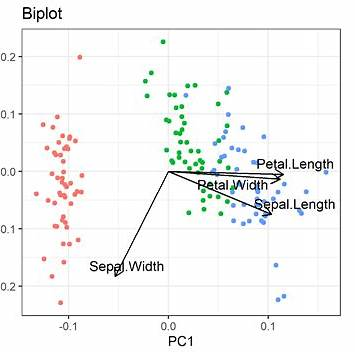
\includegraphics[width=0.6\textwidth]{imagenes/pca_biplot_genomics.png}
	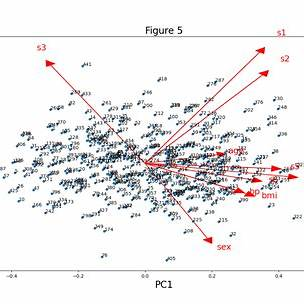
\includegraphics[width=0.6\textwidth]{imagenes/pca_biplot_genomics1.png}
\end{center}

\noindent
\textbf{Fuente:} \emph{Liu et al. (2020). ``PCA reveals the underlying patterns of RNA-Seq data in cancer studies''. Nature Communications.}

\vspace{1em}
\noindent
El PCA ayuda a identificar subgrupos celulares (p. ej., células madre, células cancerígenas) que tienen perfiles de expresión similares. Esto es clave para desarrollar terapias personalizadas.

\subsection*{PCA en Ciencia de Materiales: Análisis de Espectros Raman}

\noindent
Otra aplicación reciente del PCA está en el \emph{procesamiento de espectros Raman}, ampliamente usado para caracterizar materiales a nivel molecular. Los espectros Raman son vectores con intensidades para cada longitud de onda, generando matrices grandes (\( m \) muestras, \( n \) longitudes de onda).

\noindent
\textbf{Objetivo:} Detectar patrones de cambio en los materiales (p. ej., formación de defectos, cristalización) a partir de sus espectros.

\vspace{1em}
\noindent
\textbf{Fórmula para proyección de un espectro:}
\[
y^{(i)} = W^T (x^{(i)} - \bar{x})
\]
donde:
\begin{itemize}
	\item \( x^{(i)} \) es el espectro del material \( i \).
	\item \( \bar{x} \) es el espectro medio.
	\item \( W \) es la matriz de autovectores principales.
\end{itemize}

\vspace{1em}
\noindent
\textbf{Gráfico sugerido:} \emph{Mapa de calor de coeficientes de carga de los componentes principales}:
\begin{center}
	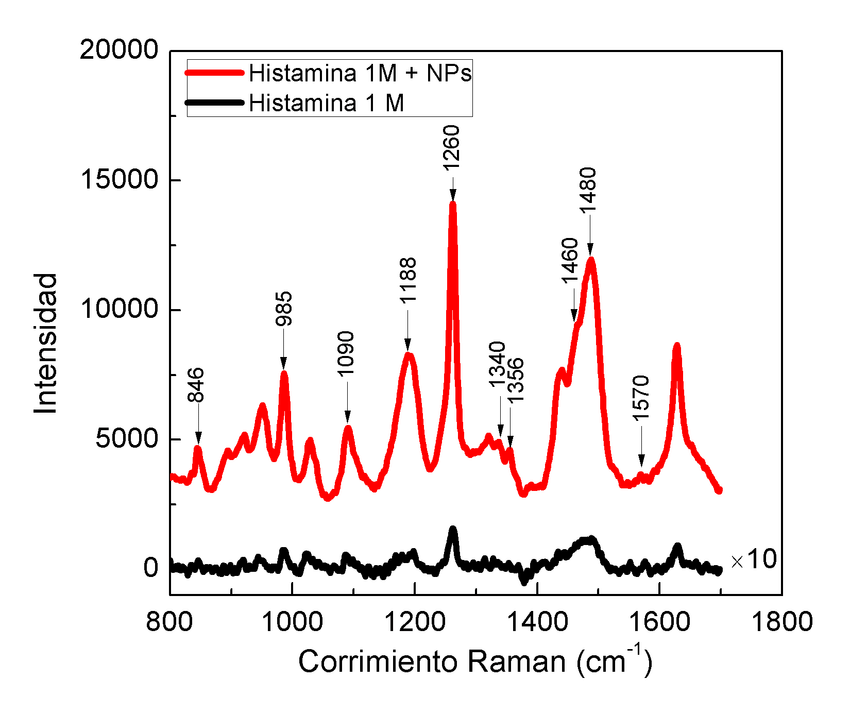
\includegraphics[width=0.65\textwidth]{imagenes/pca_raman_heatmap.png}
\end{center}

\noindent
\textbf{Fuente:} \emph{Zhao et al. (2021). ``PCA-enhanced Raman spectroscopy for defect analysis in graphene''. Advanced Materials Interfaces.}

\vspace{1em}
\noindent
\textbf{Resultados clave:} Gracias al PCA, se pueden separar \emph{zonas con defectos} y \emph{zonas cristalinas puras} en la estructura del grafeno, sin necesidad de técnicas invasivas.

\subsection*{Ventajas y Limitaciones en Estas Aplicaciones}

\textbf{Ventajas:}
\begin{itemize}
	\item Reduce el número de variables de miles a pocas decenas, facilitando el análisis.
	\item Mejora la precisión de modelos predictivos posteriores (p. ej., clasificación de cánceres o de fases de materiales).
\end{itemize}

\textbf{Limitaciones:}
\begin{itemize}
	\item El PCA asume linealidad; para datos con relaciones no lineales, métodos como \emph{t-SNE} o \emph{UMAP} pueden ser más efectivos.
	\item Requiere normalización cuidadosa para evitar sesgos.
\end{itemize}

\vspace{1em}
\noindent
\textbf{Conclusión:} Estas aplicaciones recientes demuestran la versatilidad del PCA para extraer patrones significativos en grandes volúmenes de datos biomédicos y de materiales. Sin embargo, deben considerarse sus límites cuando las relaciones no son lineales o los datos no están adecuadamente normalizados.




	\newpage
	\section{Referencias}
	\begin{itemize}
		\item Kaware, S. (2021). \emph{A Model Based Linear Algebraic Approach for Machine Learning}. IEEE.
		
		\item Alpaydin, E. (2014). \emph{Introduction to Machine Learning}. MIT Press.
		
		\item Deisenroth, M. P., Faisal, A. A., \& Ong, C. S. (2019). \emph{Mathematics for Machine Learning}. Cambridge University Press.
		
		\item Murphy, K. P. (2012). \emph{Machine Learning: A Probabilistic Perspective}. MIT Press.
		
		\item Strang, G. (2016). \emph{Linear Algebra and Its Applications}. Cengage Learning.
	\end{itemize}
	
\newpage
\section*{Anexos}
\addcontentsline{toc}{section}{Anexos}
	\textbf{Participación por integrante:}
	\begin{itemize}
		\item Koc Góngora, Luis Enrique: 100\%
		\item Mancilla Antay, Alex Felipe: 100\%
		\item Melendez Garcia, Herbert Antonio: 100\%
		\item Paitan Cano, Dennis Jack: 100\%
	\end{itemize}
	
\end{document}